\documentclass[a4paper,12pt]{article}
%%%%%%%%%%%%%%%%%%%%%%%%%%%%%%%%%%%%%%%%%%%%%%%%%%%%%%%%%%%%%%%%%%%%%%%%%%%%%%%%%%%%%%%%%%%%%%%%%%%%%%%%%%%%%%%%%%%%%%%%%%%%%%%%%%%%%%%%%%%%%%%%%%%%%%%%%%%%%%%%%%%%%%%%%%%%%%%%%%%%%%%%%%%%%%%%%%%%%%%%%%%%%%%%%%%%%%%%%%%%%%%%%%%%%%%%%%%%%%%%%%%%%%%%%%%%
\usepackage{eurosym}
\usepackage{vmargin}
\usepackage{framed}
\usepackage{amsmath}
\usepackage{graphics}
\usepackage{epsfig}
\usepackage{subfigure}
\usepackage{enumerate}
\usepackage{fancyhdr}

\setcounter{MaxMatrixCols}{10}
%TCIDATA{OutputFilter=LATEX.DLL}
%TCIDATA{Version=5.00.0.2570}
%TCIDATA{<META NAME="SaveForMode"CONTENT="1">}
%TCIDATA{LastRevised=Wednesday, February 23, 201113:24:34}
%TCIDATA{<META NAME="GraphicsSave" CONTENT="32">}
%TCIDATA{Language=American English}

\pagestyle{fancy}
\setmarginsrb{20mm}{0mm}{20mm}{25mm}{12mm}{11mm}{0mm}{11mm}
\lhead{MS4222} \rhead{Kevin O'Brien} \chead{Normal Distribution} %\input{tcilatex}

\begin{document}

%----------------------------------------------------%
\section*{Normal Distribution: Worked Example}
%\section{Exam Question:MA4413 Autumn 2008 paper}

	
		A model of an on-line computer system gives a mean times to retrieve a record from a direct access storage system device of 200 milliseconds, with a standard deviation of 58 milliseconds. If it can assumed that the retrieval times are normally distributed:
		
		\begin{enumerate}[(a)]
			\item What proportion of retrieval times will be less than 75 milliseconds?
			\item What proportion of retrieval times will be between 150 and 250 milliseconds?
			\item What is the retrieval time below which 10\% of retrieval times will be?
		\end{enumerate}
		

	\noindent \textbf{Normal Distribution Curve for $X$}
	
	\begin{center}
		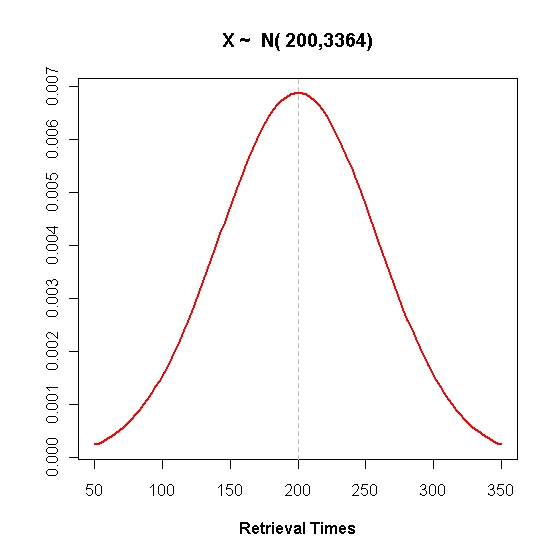
\includegraphics[scale=0.55]{images/5BNormal1}
	\end{center}



	\subsection*{Solution to Part a}
	What proportion of retrieval times will be less than 75 milliseconds?\\ \bigskip
	
	\begin{itemize}
		\item Let X be the retrieval times, with $X \sim \mbox{N}(200,58^2)$.\\
		\item The first question asks us to find $P( X \leq 75)$. \\
		\item First compute the Z-score.
		\[ X_o =  {X_o - \mu \over \sigma} = {75 - 200 \over 58}  = -2.15 \]
	\end{itemize}

	

	
	\begin{center}
		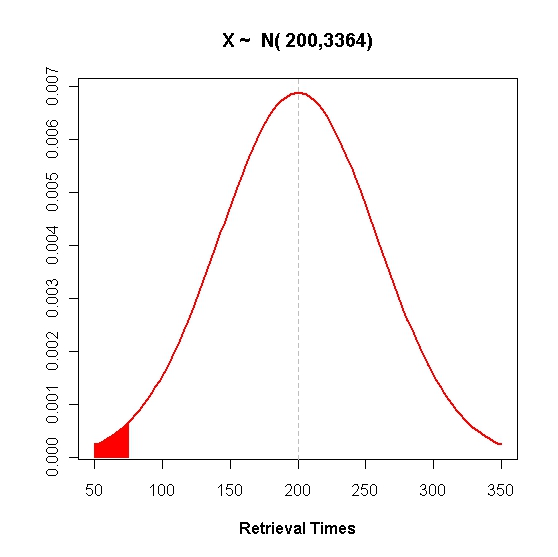
\includegraphics[scale=0.40]{images/5BNormal2}
	\end{center}
	
\noindent In this case, the probability of interest $P(X\leq 75)$, is represented by the red area under the curve.
	
	
%	\begin{itemize}
%		\item We can say
%		\[ P( X \geq 75) = P( Z \geq -2.15)\]
%		\item Using symmetry rule and complement rule
%		\[ P( Z \geq -2.15) = P( Z \leq 2.15) = 1- P( Z \geq 2.15)\]
%		\item From tables $P( Z \geq 2.15) = 0.0158$
%		\item Therefore $P( Z \leq 2.15) = 0.9842$
%		\item Furthermore $P( X \geq 75) = \boldsymbol{0.9842}$ [Answer].
%	\end{itemize}
	\begin{itemize}
		\item We can say
		\[ P( X \leq 75) = P( Z \leq -2.15)\]
		\item Using symmetry rule
		\[ P( Z \leq -2.15) = P( Z \geq 2.15)\]
		\item From tables $P( Z \geq 2.15) = 0.0158$
		%\item Therefore $P( Z \leq 2.15) = 0.9842$
		\item Furthermore $P( X \leq 75) = \boldsymbol{0.0158}$ [Answer].
	\end{itemize}
				

\newpage	

	
	\subsection*{Solution to part b}
	\begin{itemize}
		\item What proportion of retrieval times will be between 150 and 250 milliseconds?
		\item Find $P(150 \leq X \leq 250)$
		\item Use the `Too Low / Too High ' approach.
		\item Too low $P( X \leq 150)$
		\item Too high $P( X \geq 250)$
		\item Find the z-scores for each.
		\[ Z_{150} =  {150 - 200 \over 58}  = -0.86 \]
		\[ Z_{250} =  {250 - 200 \over 58}  = 0.86 \]
	\end{itemize}

%	\begin{center}
%		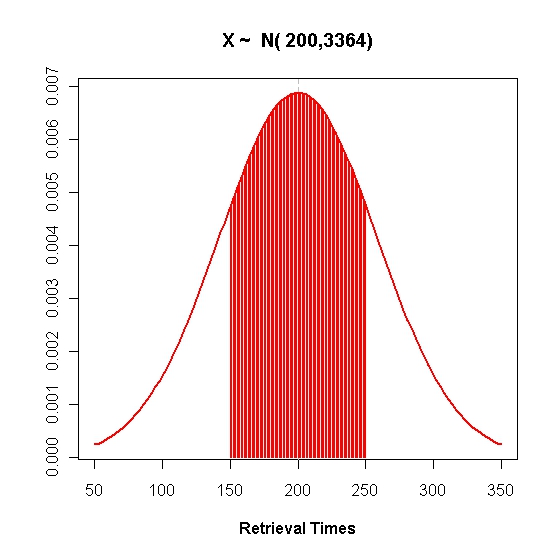
\includegraphics[scale=0.40]{images/5BNormal3}
%	\end{center}
	
	\begin{itemize}
		\item We can now say
		\begin{enumerate}
		    \item $P( X \leq 150) = P( Z \leq -0.86)$
		\item $P( X \geq 250) = P( Z \geq 0.86)$
		\end{enumerate}

		\item By symmetry rule, $P( Z \leq -0.86) = P( Z \geq 0.86)$
		\[ P( X \leq 150) =  P( X \geq 250) \]
		\item Let's compute $P( X \geq 250)$. Using tables
		\[P( X \geq 250) = P( Z \geq 0.86) = 0.1949 \]
	\end{itemize}


	
	\textbf{Using the Interval Rule}
	\begin{itemize}
		\item Too high: $P( X \geq 250) = 0.1949 $
		\item Too low:  $P( X \leq 150) = 0.1949 $
		\item Probability of being inside interval:
		
		\[ P(150 \leq X \leq 250) = 1- [ P( X \leq 150) + P( X \geq 250)] \]
		
		\item $P(150 \leq X \leq 250) = 1- [ 0.1949 + 0.1949 ] = \boldsymbol{0.6102}$
		
	\end{itemize}	
	
\subsection*{Solution to part c}
	\begin{itemize}
		\item What is the retrieval time below which 10\% of retrieval times will be?
		\item Find $A$ such that $P(X \leq A) = 0.10$.
		\item What Z-score would correspond to $A$? Lets call it $Z_A$.
		\item $P(Z  \leq Z_A) = 0.10$
		\item Remark: $Z_A$ could be negative.
		\item Using symmetry $P(Z \geq -Z_A) = 0.10$.
		\item Remark: $-Z_A$ could be positive.
	\end{itemize}


	
%\begin{center}
%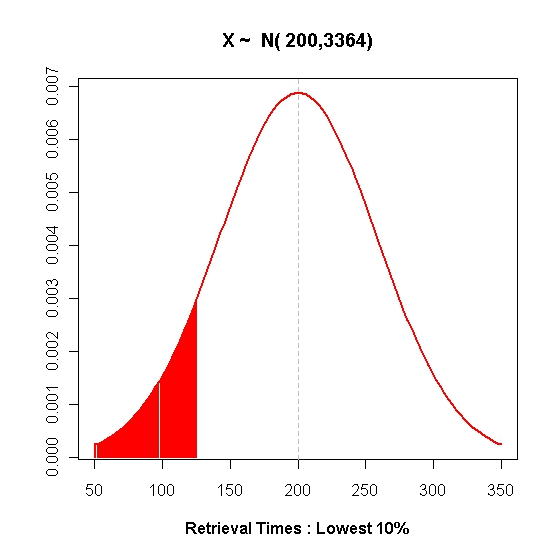
\includegraphics[scale=0.40]{images/5BNormal4}
%\end{center}
	

	\begin{itemize}
		\item Use the Murdoch Barnes tables to get an approximate value for $-Z_A$.
		\item The nearest value we can get is 1.28. ( $P( Z \geq 1.28) = 0.1003$ ).
		\item If $-Z_A = 1.28$, then $Z_A=-1.28$
		\item We can now say
		\[ P(X \leq A) = P(Z \leq -1.28) \]
		
	\end{itemize}

	\begin{itemize}
		\item Necessarily $A$ and $Z_A$ are related by the standardization formula
		\item Recall that $\mu = 200$ and $\sigma = 58$.
		\[ -1.28  = {A - 200 \over 58} \]
		\item Re-arranging (Multiply both sides by 58).
		\[ -74.24  = A - 200 \]
		\item Re-arranging again (Add 200 to both sides).
		\[ 125.76 =  A \]

		\item Now we know the retrieval time below which 10\% of retrieval times will be.
		\item $P(X \leq 125.76) = 0.10$ [Answer].
	\end{itemize}

\end{document}
